In this section, we empirically evaluate STOIC's performance when executing machine learning application. For every request, we run benchmark application on all available runtimes and compare the selection made by STOIC based on the predicted latency and the runtime with least total latency. In this section, we first describe the benchmark application that we consider, followed by our experimental setup and results. 

\subsection{Benchmark Application and Dataset}

We evaluate STOIC using an image processing application that classifies animal images from a wildlife monitoring system called ``Where's The Bear" (WTB)~\cite{ref:wtb}. ``Where's The Bear" is an end-to-end distributed data acquisition and analytics system that implements an IoT architecture and edge cloud. Our application makes inferences for each photo taken by deployed camera traps in Sedgwick Natural Reserve using a convolutional neural network (CNN)~\cite{ref:cnn}.  We train the model using labeled images from the WTB dataset. Technically, the application employs Tensorflow and Scikit-learn~\cite{ref:scikit} to implement image classification.  

In total, there are five classes that we consider in the CNN model training: Bird, Fox, Rodent, Human and Empty. Since class size is unbalanced due to frequencies of animal occurrences, we up-sample minority classes (e.g. fox) using the Keras ImageDataGenerator~\cite{ref:keras}.  Doing so ensures that the classification model is not biased. We resize every image in the WTB dataset to $1920 \times 1080$, and for each class, the dataset contains 251 images used to train the CNN model. Once model training is complete, the application stores this model in hdf5 format in cloud storage at both edge cloud (disk storage) and Nautilus (a shared volume in a Ceph file system).

To better harness the multiple GPU runtime in the public cloud, the application assigns each GPU to a spawned process, namely worker, and adds all images in the batch to a shared asynchronous queue. Upon the execution, all workers pick up the image job from the shared queue until it is exhausted. This mechanism ensures multiple GPUs evenly divide the workloads and achieve quasi-linear acceleration at application level, where the perfect linear speed-up is unattainable due to model loading and memory transfer overhead~\cite{ref:multi_gpu}. 

\subsection{Efficacy Experiments}

We first test the efficacy of STOIC by processing a sequence of image batches at four runtimes individually and then compare them with the determined runtime by STOIC. According to 2016 WTB dataset, the size of image batch fits to normal distribution $\mathbf{N}(\mu = 42.75, \sigma^2 = 39.5)$. To conduct an unbiased evaluation, we seed the simulator to make these image batches consistent across all runtimes and STOIC.


To make the result reliable, we conduct the experiment for a 24-hour time range, in which  154 image batches (616 executions) are processed by STOIC. Based on the data we observe, STOIC successfully selects the runtime of least latency by \textbf{85.1\%} of times (131 out of 154). We then compare the actual latency between the worst selection scenario and STOIC. The total latency of selected runtime by STOIC is 8041.06 seconds, whereas in the worst scenario the total latency is 18563.82 seconds. This indicates STOIC accelerates the execution of image processing by \textbf{2.3} times if the runtimes are erroneously selected by dispatcher.

\begin{figure}[t] \centering 
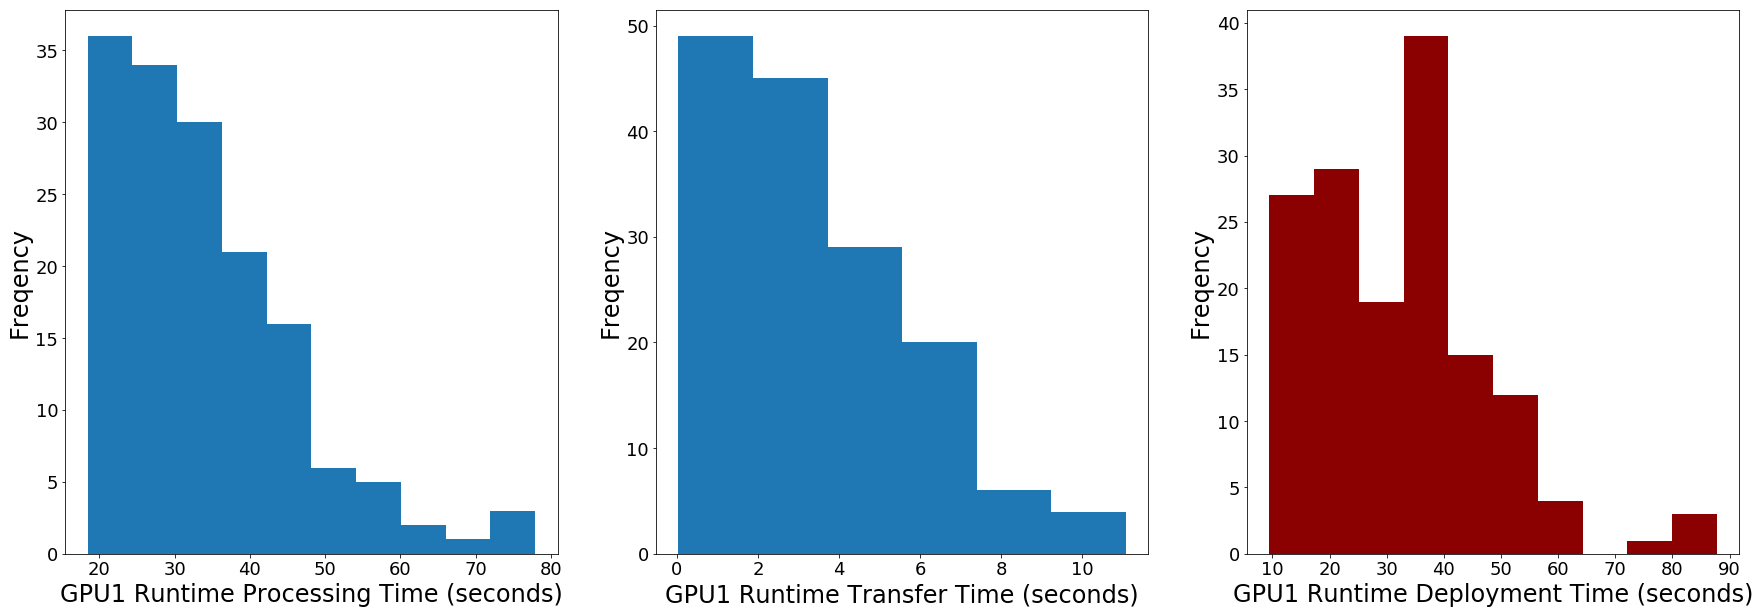
\includegraphics[scale=0.14]{gpu1_latency.png}
\caption{The distribution of three components in total response time~($T_r$): Processing time ($T_p$), Runtime deployment time ($T_d$) and Transfer time ($T_t$). The x-axis represents the time range, while the y-axis is the frequency of executions. The deployment time, which is depicted in the red histogram, is volatile and error-prone to prediction.
\label{fig:breakdown}}
\end{figure}

We further analyze the data points where STOIC made erroneous selection and found two sources of error. First, the most error occurs around two batch sizes where the total response time of runtimes have approximately same latency. To be specific, the edge and GPU runtimes cross over at 35 image batch size, and 90 image batch size for the GPU1 and GPU2 runtimes. At these cross-points, the close predictions of latency lead to incorrect selection. Second, the deployment time for GPU runtimes are volatile and error-prone to prediction. As a representative instance, Figure~\ref{fig:breakdown} demonstrates the distribution of processing time ($T_p$), transfer time ($T_t$) and deployment time ($T_d$) of GPU1 runtime. We observe geometric distribution from the histogram of processing time and transfer time, whereas deployment time varies irregularly with many outliers. These two phenomenons lead to mistaken selections in the experiment.

Further, we define an error metric, Mean Deadline Error (MDE), to better gauge the predictive capability of STOIC between edge cloud and GPU runtimes. Since the dedicated edge cloud is closer to the data source and more homogeneous and robust compared to public cloud, we are only concerned when GPU runtimes have longer total latency than edge cloud and STOIC deploys the workload to GPU runtimes. Mean Deadline Error is defined as $MDE = \frac{1}{n}\sum(L_g - L_e) \,|\ if \ L_g > L_e \ \& \ R_s = GPUx $, where $L_g$ is the latency of GPU runtime, $L_e$ is the latency of edge cloud, $R_s$ is the selected runtime by STOIC. Based on the experiment data, the MDE gpu1 is \textbf{26.68} seconds (44.18\% to the mean gpu1 runtime latency) and MDE gpu2 is \textbf{43.98} seconds (47.43\% to the mean gpu2 runtime latency). This result implies that the unstable deployment time of GPU runtimes significantly affects the accuracy of prediction made by STOIC. 

\begin{figure}[t] \centering 
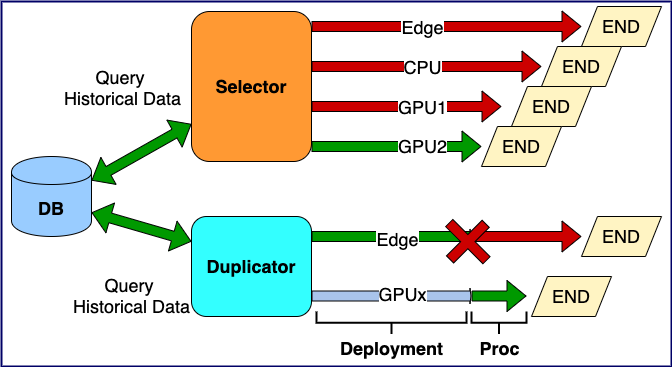
\includegraphics[scale=0.35]{selector_duplicator.png}
\caption{The selector and duplicator modes of STOIC. 
\label{fig:duplicator}}
\end{figure}

To address the above issue, we reconfigure STOIC into the duplicator mode demonstrated in Figure~\ref{fig:duplicator}. Based on the historical data, the selector makes prediction and only execute workload at the runtime with least total latency, whereas the duplicator runs workload on edge cloud and GPU runtimes concurrently, and halts the edge cloud execution if the remaining time at edge cloud is longer than the expected processing time ($T_p$) at the GPU runtime once it completes deployment. Under this mode, STOIC is able to make right selection between edge cloud and GPU1 runtime and promptly respond to the request \textbf{96.7\%} of times (149 out of 154). 

\begin{table}[t] 
\centering
\captionsetup{justification=centering}
\caption{ \hspace{0pt} \\
\textsc{Mean and Stdev. of Total Response Time~($T_r$) and Processing Time~($T_p$) of 40-Image Batch: STOIC Schedules Tasks onto the Runtime (\textit{gpu1}) that Has the Least Total Response Time~($T_r$).}}
\scriptsize
\resizebox{\columnwidth}{!}{
\begin{tabular}{|c|c|c|c|} 
\hline
& \textbf{Success Rate} & \textbf{Avg. Latency (sec)} & \textbf{Speedup}\\
\hline
Selector 4 runtimes & 85.1\% & 52.21 & 2.30x \\
\hline
Duplicator Edge vs GPU1 & 96.7\% & 51.15 & 2.35x \\
\hline
Duplicator Edge vs GPU2 & \textbf{94.8}\% & \textbf{50.86} & \textbf{2.37x} \\
\hline
\end{tabular}
}

\label{tab:validation}
\end{table}


In the case of gpu2 runtime, it has more variable deployment and processing time compared to gpu1 runtime, which possibly leads to lower success rate of selection. The analytics of the data proves this assumption that STOIC makes right selection between edge cloud and gpu2 runtime by \textbf{94.8\%} (146 out of 154) of times, 1.9\% lower than being with gpu1 runtime. However, the average latency of gpu1 runtime (154 image batches) is \textbf{57.61} seconds, whereas the total latency is \textbf{54.52} seconds for gpu2 runtime. We argue that even though STOIC make more mistakes for gpu2 than gpu1, the duplicator mode of edge cloud versus gpu2 makes the entire end-to-end system faster and more efficient. We plan to investigate runtimes with more GPUs and the trade-off between the predictability and efficiency of system as future work.
